\documentclass[10pt]{article}
\usepackage[T1]{fontenc}
\usepackage[a4paper,margin=24mm]{geometry}
\usepackage{amsmath,amssymb,amsthm,mathtools,microtype}
\usepackage{graphicx}
\usepackage[hidelinks]{hyperref}
\newcommand{\Q}{\mathbb Q}\newcommand{\Z}{\mathbb Z}
\DeclareMathOperator{\den}{den}\DeclareMathOperator{\rank}{rank}
\newtheorem{theorem}{Theorem}\newtheorem{corollary}[theorem]{Corollary}
\title{Two global traces recover rational Erd\H{o}s--Straus denominators}
\author{The Clankers}
\date{20 September 2026}
\begin{document}\maketitle
\begin{abstract}
If $n\ge3$ positive rational numbers have reciprocal sum $4/p$, their first
$n-1$ power sums are integers exactly when all the numbers are integers. For the
three-denominator equation, two traces suffice. We prove a more general
common-denominator law, then give a one-trace return and complete coefficient
fibres on the original integer gate source. This is a global integrality test,
not a proof that the relevant source is occupied at every prime.
\end{abstract}

\begin{theorem}\label{th:den}
Let $x_1,\ldots,x_n\in\Q^\times$, $n\ge2$, and suppose their power sums
$s_k=\sum_i x_i^k$ are integers for $1\le k<n$. If their nonzero reciprocal sum is
$m/b$ in lowest terms, $b>0$, then all reduced denominators are the same integer
$d$, and
\[
 \boxed{\gcd(d,b)=1,\qquad d^n\mid(n-1)!m.}
\]
If $n$ is odd, $d$ is odd.
\end{theorem}
\begin{proof}
For elementary symmetric functions $e_j$, Newton's identities
$j e_j=\sum_{k=1}^j(-1)^{k-1}e_{j-k}s_k$ give $j!e_j\in\Z$ for $j<n$.
They follow by taking the formal logarithmic derivative of
$\prod_i(1+x_iT)$; see Euler [1, \S\S3,5--7].
At a denominator prime $\ell$, suppose the minimum root valuation is $-a<0$
and exactly $r<n$ roots attain it. Their product is the unique least-valuation
term of $e_r$, so $v_\ell(e_r)=-ar$. But
$v_\ell(e_r)\ge-v_\ell(r!)>-r\ge-ar$, a contradiction. Hence every root has
the same negative valuation at every denominator prime, proving the common
reduced denominator assertion.
Writing $x_i=A_i/d$ with each $A_i$ a unit at primes of $d$, use
$e_{n-1}=(m/b)e_n$ and $e_n=\prod_iA_i/d^n$. At $\ell^a\parallel d$ this gives
\[
 na\le v_\ell((n-1)!)+v_\ell(m)-v_\ell(b).
\]
The factorial valuation is less than $n$, so $\ell\mid m$ and $\ell\nmid b$.
The divisibility follows. If $n$ were odd and $d$ even, the scaled sum of its
$n$ odd reduced numerators would be odd, contradicting $s_1\in\Z$.
\end{proof}

\begin{corollary}\label{cor:es}
For $n\ge3$, $p\in\Z_{>0}$ and $x_i\in\Q_{>0}$ with $\sum_i1/x_i=4/p$,
\[
 \boxed{(x_1,\ldots,x_n)\in\Z^n
 \quad\Longleftrightarrow\quad(s_1,\ldots,s_{n-1})\in\Z^{n-1}.}
\]
In particular two integral traces suffice for the Erd\H{o}s--Straus equation.
\end{corollary}
\begin{proof}
The reduced reciprocal numerator divides four, so Theorem~\ref{th:den} excludes
odd denominator primes. Odd $n$ excludes two. For even $n\ge4$, $n-1$ has at
least two nonzero binary digits, so
$v_2((n-1)!)+2=n+1-s_2^{\rm bin}(n-1)\le n-1$; this also excludes two.
The converse is immediate. For $n=2$ the statement fails at $(p/2,p/2)$ with odd $p$.
\end{proof}

The numerator matters: $(1/3,1/3,4/3)$ has first two traces $(2,2)$ and
reciprocal sum $27/4$. The full source edition further proves that at $n=3$ the
possible common denominator is exactly an odd $d$ with $v_3(d)\le1$ and every
other prime factor $1\pmod3$, and constructs all such denominator types.

\section*{A single trace on the original integer gate}
Let $p\equiv1\pmod4$ be prime, $p/4<a<p/2$, $R=4a-p$. Before imposing a divisor
budget, take a positive integer $U$ with $R\mid a+U$ and set
\[
 (x,y,z)=\left(a,\frac{pa(U+a)}{RU},\frac{p(a+U)}R\right),
 \qquad S=p+x+y+z.
\]
This is a positive rational ES identity, with $z\in\Z$. Because $R$ is a unit
modulo $U$, its exact trace denominator is
\[
 \boxed{\den S=\frac{U}{\gcd(U,pa^2)}.}
\]
Indeed the integral numerator $pa(U+a)/R$, reduced modulo $U$, has the same gcd
with $U$ as $pa^2$. Thus an integral trace gives exactly $U\mid pa^2$.
At $v_p(U)=0$ it returns the original M divisor $u=U$; at $v_p(U)=1$ it returns
the original E divisor $u=U/p$. The gate in the latter case becomes $4u+1=0$
modulo $R$. These are the original Type-I/II coordinates [2, \S2], not a new
parametrization.

Explicitly, with $g=\gcd(a,u)$, set $h=g^2/u$, $r=u/g$, $s=a/g$.
For M, $\lambda=(r+s)/R$ returns $(a,phs\lambda,phr\lambda)$; for E,
$\kappa=(pr+s)/R$ returns $(a,hs\kappa,phr\kappa)$. Their ordered inverses are
$pa^2/(Ry-pa)$ and $a^2/(Ry-pa)$. The original exponent of each prime is recovered
from $u$. An integral trace has tag M precisely when $S\equiv a\pmod p$.

Let $\Omega=\{1\le U\le pa^2:R\mid a+U\}$, $\Theta=\{S(U):U\in\Omega\}$,
and let $\Phi:\Z^\Omega\to\Z^\Theta$ send each original word to its trace label.
The identity
\[
 S(U)-S(V)=\frac pR(U-V)\left(1-\frac{a^2}{UV}\right)
\]
proves that its only two-point fibres are the original middle complements
$U,V=a^2/U$. The fixed point $U=a$ is excluded by $R\nmid2a$. Exterior traces
and nonintegral traces have singleton fibres. Hence, retaining both middle
orientations,
\[
 \boxed{\rank\ker\Phi=|M_a|/2,\qquad
 |\Theta\cap\Z|=|E_a|+|M_a|/2.}
\]
The actual kernel basis is $e_U-e_{a^2/U}$ for $U<a$ in M. Original integer
multiplicity two is not replaced by its zero reduction modulo two.

\begin{figure}[htbp]
\centering
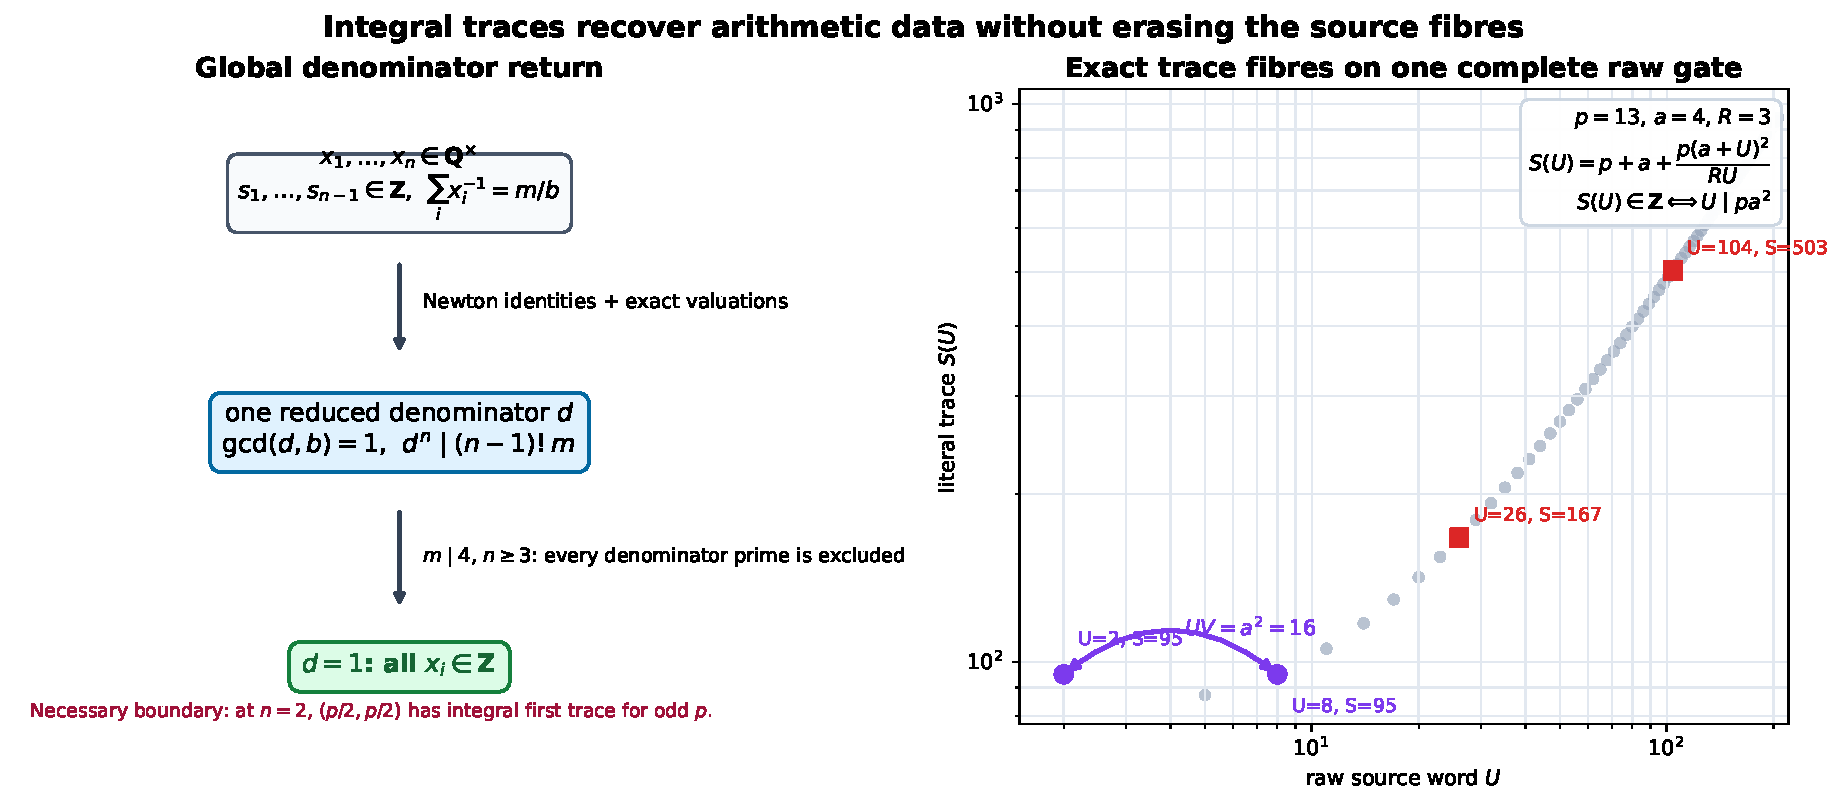
\includegraphics[width=\textwidth]{figures/trace_integrality_fibres.pdf}
\caption{Left: the exact implication proved by the common-denominator theorem,
including the necessary $n=2$ boundary. Right: the complete raw gate at
$p=13$, $a=4$, $R=3$. The four integral returns are $U=2,8,26,104$;
$U=2$ and $U=8$ form the unique two-point fibre because $UV=a^2=16$,
while the two exterior returns are singletons. Every grey point is a retained
raw word, so the diagram displays rather than removes the trace kernel.
The script \texttt{figures/trace\_integrality\_fibres.py} computes every
plotted value with exact rational arithmetic.}
\label{fig:trace-integrality-fibres-short}
\end{figure}

\section*{The first trace alone and the rationality hypothesis}
Without the full integer gate, an integral trace can leave a square-part defect.
For positive rational tails with $1/y+1/z=R/(pa)$ and $N=y+z\in\Z$, the two
reduced denominators are the same $d$. From $yz=Npa/R$ and $\gcd(pa,R)=1$,
\[
 \boxed{d^2=R/\gcd(R,N),\qquad \den(a^2+y^2+z^2)=d^2.}
\]
The second equality uses odd $R$. Thus squarefree $R$ suffices, but at the hard
prime $1009$ the exact rational identity
\[
 (x,y,z)=(286,6413/3,168238642/3)
\]
has first trace $56081971$ and second trace $28304240703866897/9$.

Rational roots are essential in Corollary~\ref{cor:es}. Let $b_1,b_2,b_3$ be the
roots of $T^3-6T^2+8T-2$. Opposite signs at $0,1,2,5$ prove there are three
positive roots. Reduction modulo three has no root, so the cubic is irreducible.
The algebraic-integer denominators $pb_i$ satisfy $\sum_i1/(pb_i)=4/p$ and have
all power traces integral, beginning with $6p$ and $20p^2$, but none is rational.
The full source edition constructs a stronger such family at every hard prime,
with an integer first denominator and the original middle prime-local cluster
signature. It is outside the rational-source domain, not an ES counterexample.

The remaining assertion is that some original shell has an integral trace in
$\Omega$ (equivalently an original E or M divisor hit). No uniform positive
lower bound on that count or kernel has been proved here. The work is an exact
global integrality return, not universal source occupancy or a completed Turn 7.

\begin{thebibliography}{2}\small
\bibitem{Euler} Euler, L. (1750/2007). \emph{A double demonstration of a theorem of
Newton, which gives a relation between the coefficient of an algebraic equation
and the sums of the powers of its roots} (J. Bell, Trans.). E153; arXiv:0707.0699,
\S\S3,5--7. Classical Newton identities; the proof above is self-contained.
\bibitem{ET} Elsholtz, C., \& Tao, T. (2013). Counting the number of solutions to
the Erd\H{o}s--Straus equation on unit fractions. \emph{Journal of the Australian
Mathematical Society, 94}, 50--105. arXiv:1107.1010, \S2, Propositions 2.2 and 2.6.
\end{thebibliography}
\end{document}
